\documentclass{standalone}
\usepackage{mathpazo}
\usepackage{siunitx}
\usepackage[american voltages, american currents, american inductors]{circuitikz}
\usetikzlibrary{calc}
\newcommand*{\equal}{=}

\begin{document}
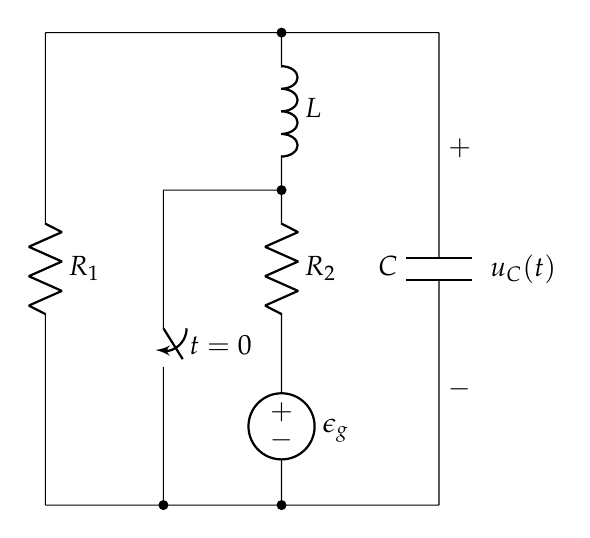
\begin{tikzpicture}
  \coordinate (A) at (0,6);
  \coordinate (B) at (3,6);
  \coordinate (C) at (5,6);
  \coordinate (D) at (0,0);
  \coordinate (E) at (3,0);
  \coordinate (F) at (5,0);
  \draw
  (A) to [short, -*] (B) to [short] (C)
  (D) to [short, -*] (E) to [short] (F)
  (A) to [R, l = $R_1$] (D)
  (B) to [L, l = $L$] ++(0, -2) coordinate (B2)
  to [R, l = $R_2$] ++(0,-2)
  to [V, l = $\epsilon_g$] (E)
  (C) to [C, l_= $C$, v^= $u_C(t)$] (F)
  (B2) to [short, *-] ++(-1.5, 0) coordinate (B3)
  to [closing switch, -*, l = $t\equal 0$] (B3|-E);
\end{tikzpicture}
\end{document}